\chapter[Onset Classification]{Onset Classification}

\section{Method}
Since forecasting actual values for \req\ is not always viable or accurate, an attempt was made to model \req\ event onsets as a classification problem whereby an onset timestep (the one in which the 20 $amu/cm^3$ threshold was crossed) was defined as a ``1", and any other time defined as a ``0". \cite{Denton2016}, which also uses the inferred \req\ from GOES Alfvén waves, indicates that daily averaged Kp and \f\ both are involved in driving the behavior of \req. By then passing relevant measurements such as Kp, $F_{10.7}$, and $V_{SW}$ into a non-linear classification model such as \texttt{patternnet} \citep{MATLAB:2014}, a predictive classification could be made based on these conditions. 

Two formats and two time scales were tested: one format consisting of passing in an entire timeseries, where each prediction was based on a sliding window of the current and previous three timesteps as one set of inputs. The other format only considered time periods at and three hours before onset, but treated each time step as its own input and classification. Both formats  are diagrammed in Figure \ref{fig:ClassifyDiagram}. The top diagram shows the classification method where the modeling window slides across one timestep at a time and only spans four timesteps at each onset. The bottom diagram depicts the prediction method where the window slides across all data, and each block of four timesteps attempts to predict an onset one step ahead. Both methods were used to make models for the two time scales of hourly and daily medians of values. 

\begin{figure}[htp!]
	\centering
	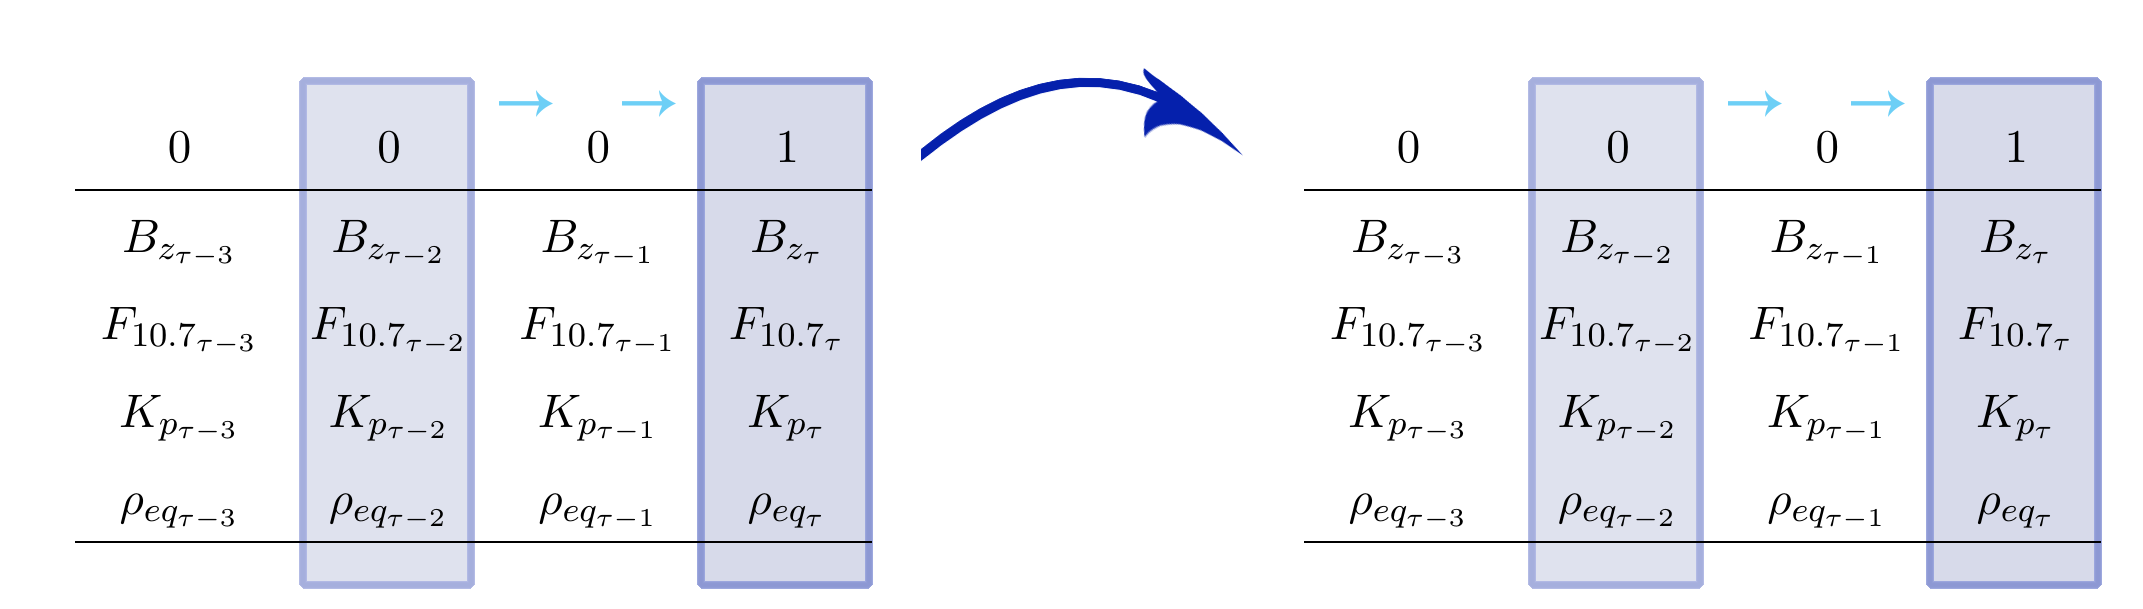
\includegraphics[width=1\linewidth]{Figures/CH5/ClassifyGraphic2.png}
	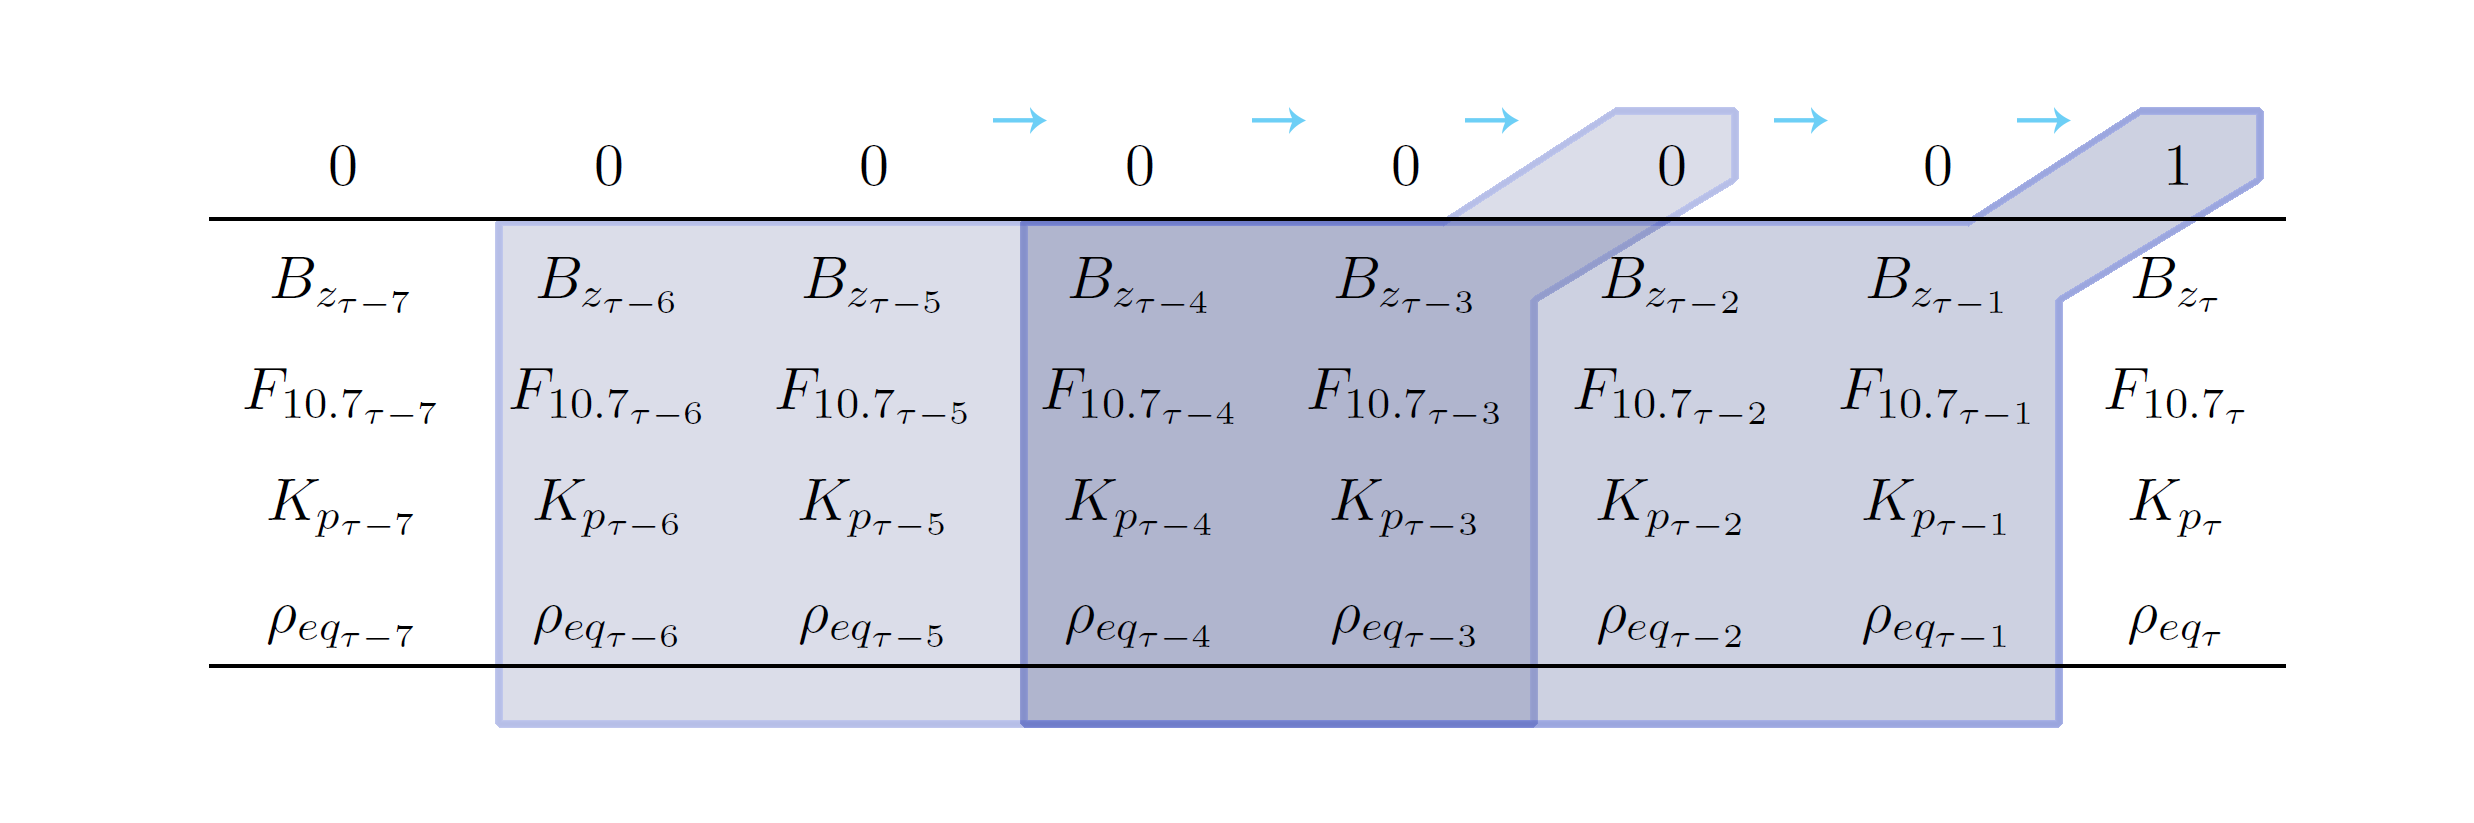
\includegraphics[width=1\linewidth]{Figures/CH5/FullGraphic.png}
	\caption{Diagram of classification (top) and prediction (bottom) methods.}
	\label{fig:ClassifyDiagram}
\end{figure}


In order to aid the model in finding event onsets despite being numerically overwhelmed by non-onsets, the targets are weighted to more highly value a "1". Since the number of events is similar between hourly and daily timescales, but the number of data points is a factor of 24 larger for the hourly scale. As such, the weights are scaled so targets have a value of the logarithm of the number of data points divided by the number of onsets, while all other points have a weight of 1. This gives a typical relative weight of 2-7 for onsets vs non-onsets. 


\section{Results}

\subsection{Classification} \label{sec:ClassifyResults}

Figure \ref{fig:OnsetEvents} is a confusion matrix, where onsets (class "1") and non-onsets (class "0") are categorized based on their real value labeled "Target Class", and the value categorized by the model labeled "Output Class". So for example, on a daily timescale, there were 582 event onsets (sum of Target class 1), and the model correctly classified 473 of them (intersection of target class 1 and output class 1). Since this classification model is primarily concerned with correctly classifying onsets, the percentage values given will be for the percent of correctly classified onsets out of the total number of onsets, shown as the green value in the bottom of column 2. This specific figure shows that trying to classify events on an hourly timescale using only the onset hour and three hours before leads to a model that classifies almost no onsets. Using daily values, however, results in a model where a full 80\% of the onsets are correctly detected and classified, but only half of the predicted onsets were actually onsets.

\begin{figure}[htp!]
	\centering
	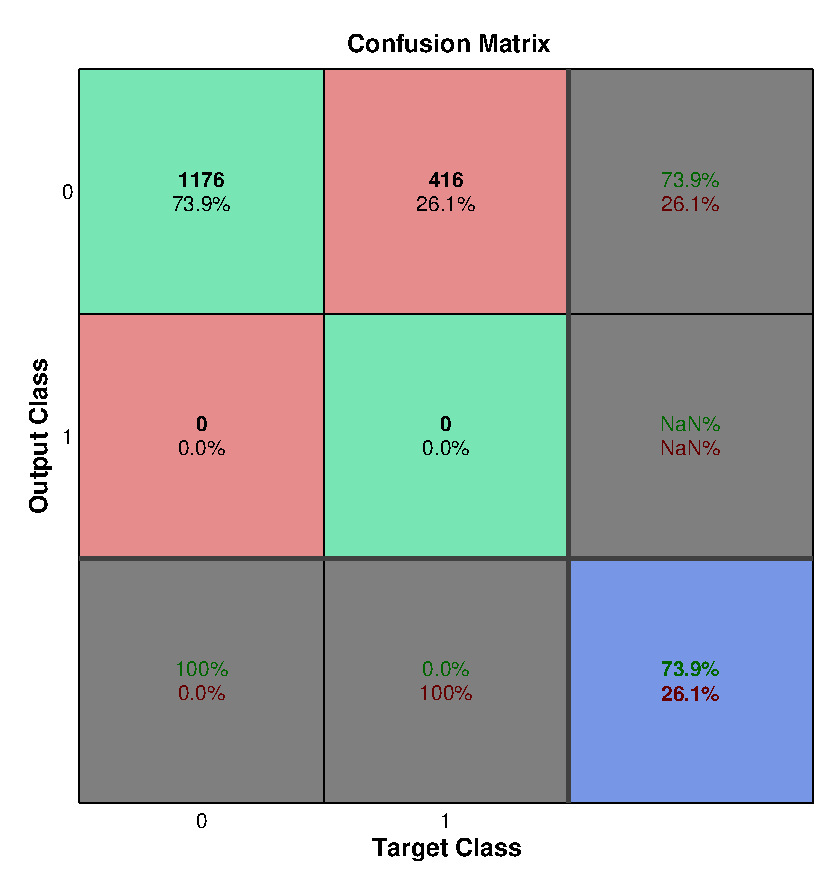
\includegraphics[width=0.45\linewidth]{Figures/CH5/NNBinaryOnset-hourly.eps}
	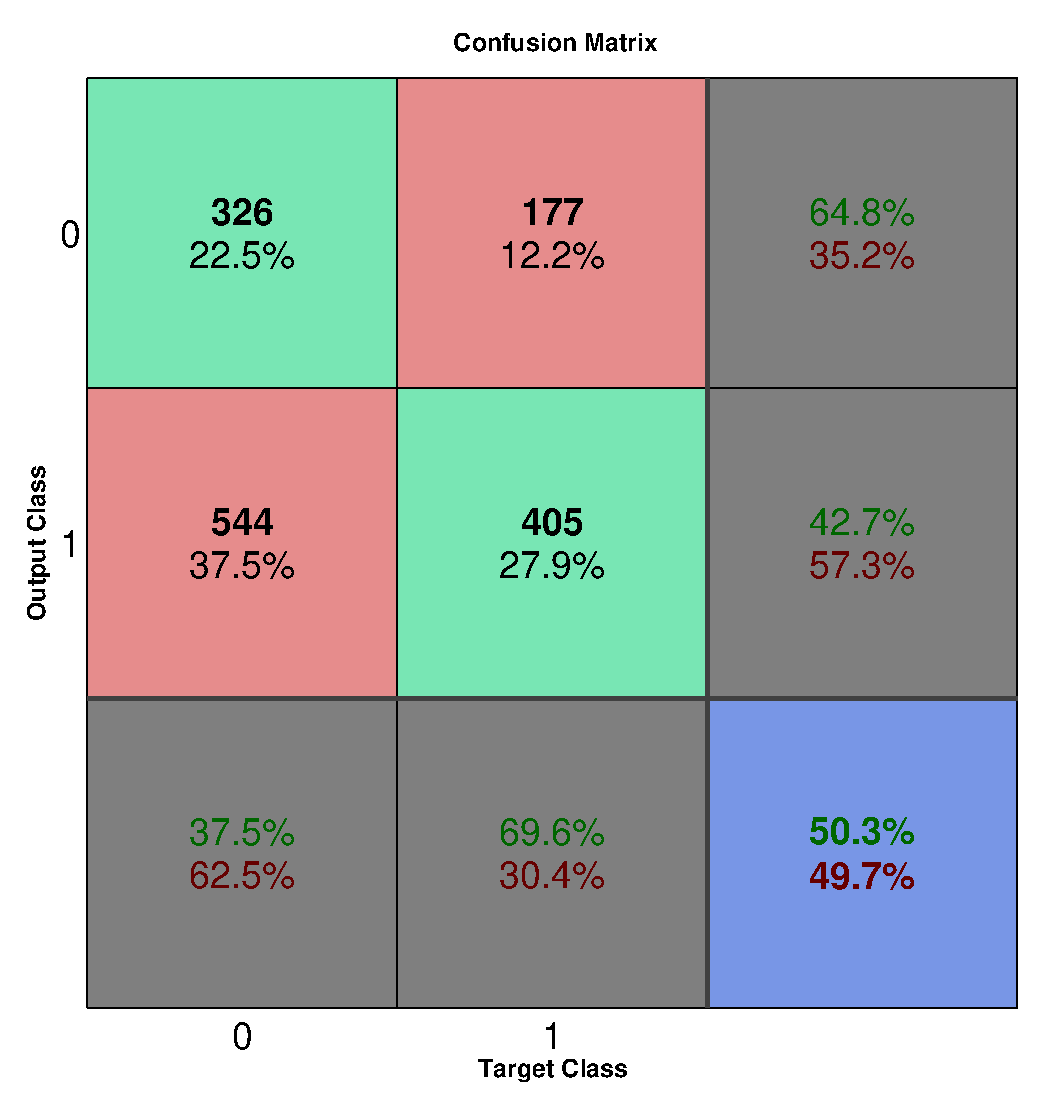
\includegraphics[width=0.45\linewidth]{Figures/CH5/NNBinaryOnset-daily.eps}
	\caption{Prediction confusion matrix for hourly (left) and daily (right) \req\ onset events using classification method.}
	\label{fig:OnsetEvents}
\end{figure}

In an attempt to find out what conditions best lead to a correct classification, histograms were made of the conditions associated with a correctly classified onset vs those of an undetected onset. Figure \ref{fig:OnsetEventsHist} shows this for the four variables used.

\begin{figure}[htp!]
	\centering
	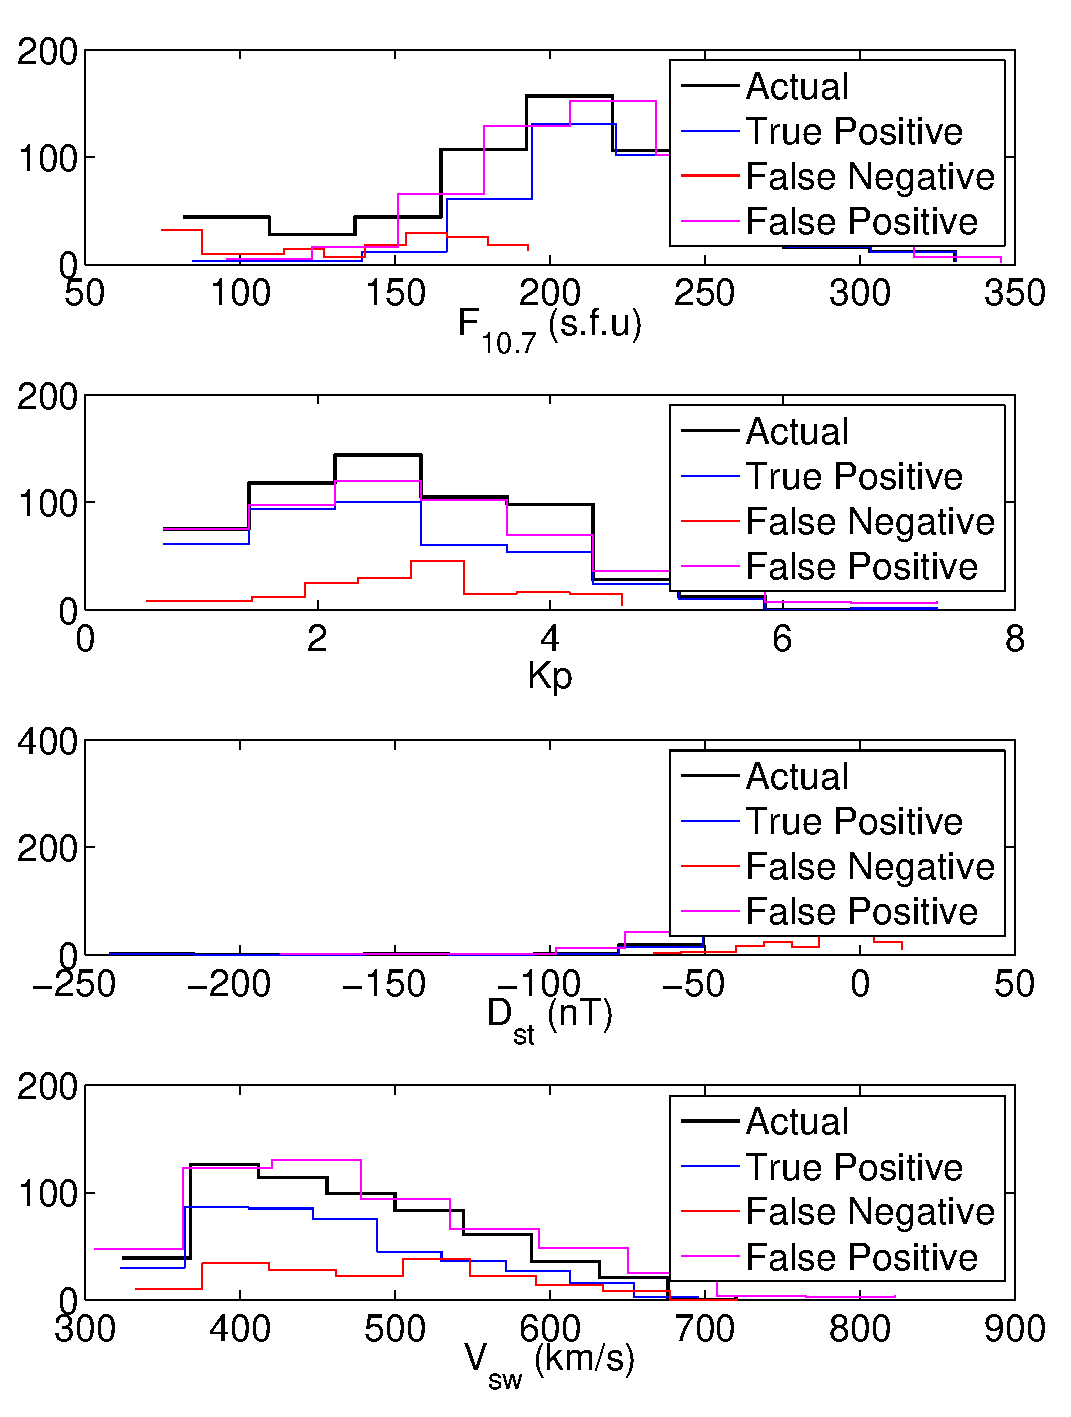
\includegraphics[width=0.85\linewidth]{Figures/CH5/NNBinaryOnset-daily-hist.eps}
	\caption{Histogram of onset conditions for daily-averaged \req\ events binned by correctness of prediction.}
	\label{fig:OnsetEventsHist}
\end{figure}

It shows that the model tended to miss onsets during periods of particularly low \f, and during high speed solar winds, but was largely unaffected otherwise.

The next test was to add more obvious indicators of an event onset, such as the data being used to define an onset, and see if the model could pick that up. By adding \req\ as a factor in classifying \req\ events, the model unsurprisingly does very well, as shown in Figure \ref{fig:OnsetWithreq}.

\begin{figure}[htp!]
	\centering
	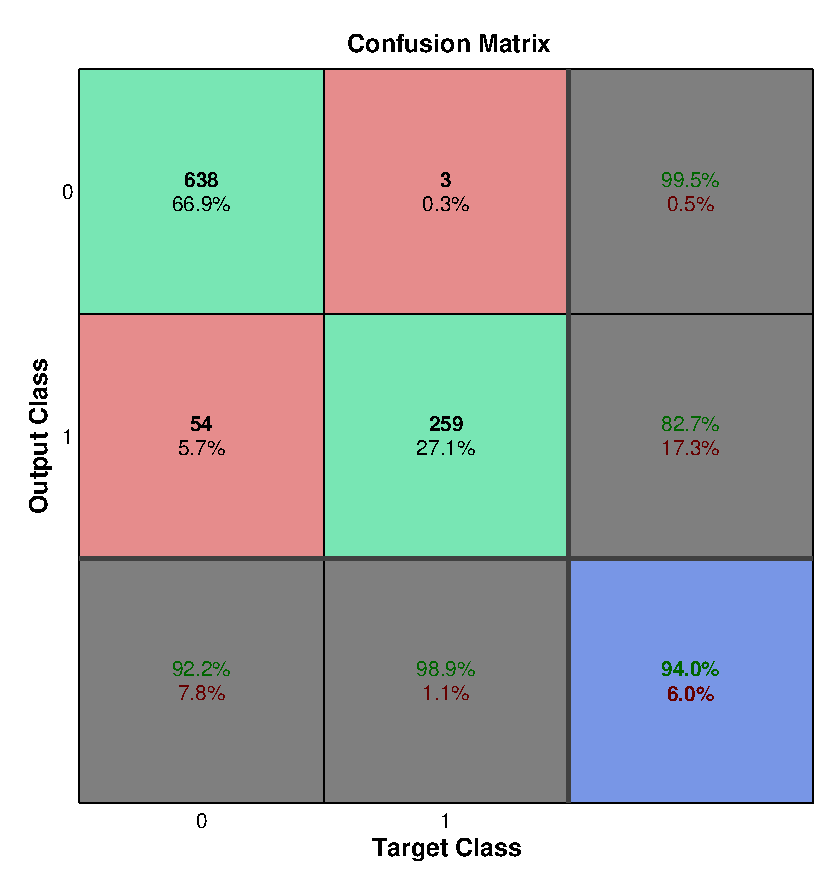
\includegraphics[width=0.45\linewidth]{Figures/CH5/NNBinaryOnset-hourly-withreq.eps}
	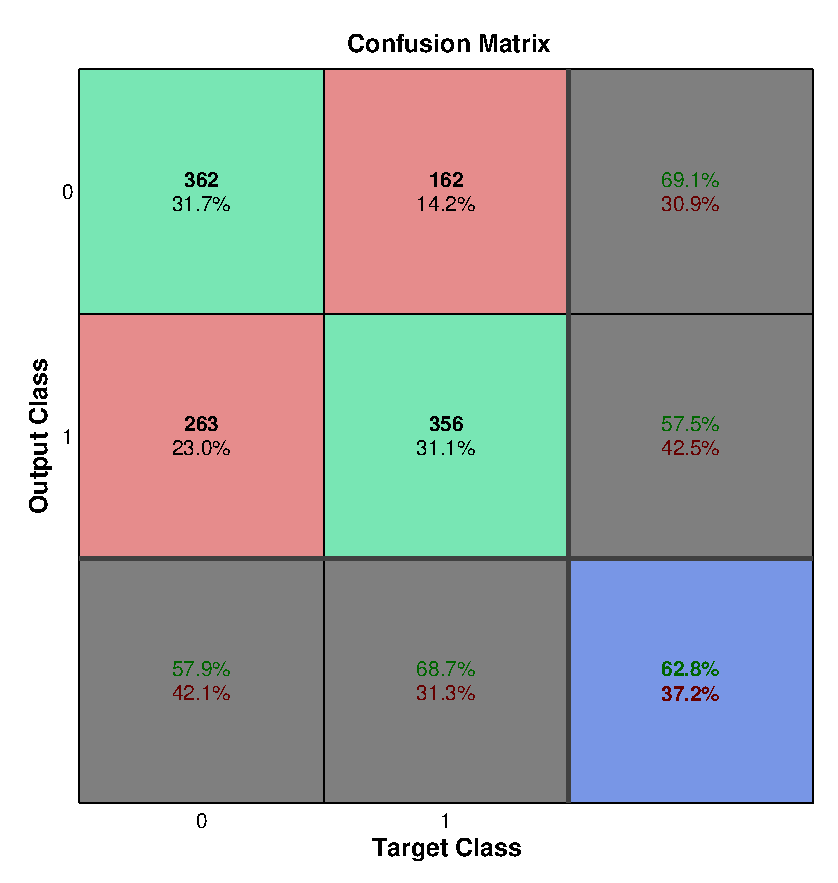
\includegraphics[width=0.45\linewidth]{Figures/CH5/NNBinaryOnset-daily-withreq.eps}
	\caption{Prediction confusion matrix for hourly (left) and daily (right) \req\ onset events, including \req\ as an input variable, and only looking at three hours before and including onset.}
	\label{fig:OnsetWithreq}
\end{figure}

With a successful true positive classification rate of 99\% and 84\% for hourly and daily 4-hour models respectively, it can be said that including \req\ information makes the models effective for classifying event onset, both validating the model as being able to determine our selection criteria as well as showing the extent to which daily averaging can obscure conditions attributed to an event. Since the \req\ events have a median duration of 14 hours above the $-20$~nT threshold, it is clear that they significantly impact the entire day enough to still be detectable. A histogram of these variables binned by true positive and false negative shows no particularly compelling trends, as seen in Figure \ref{fig:OnsetWithreq-hist}.


\begin{figure}[htp!]
	\centering
	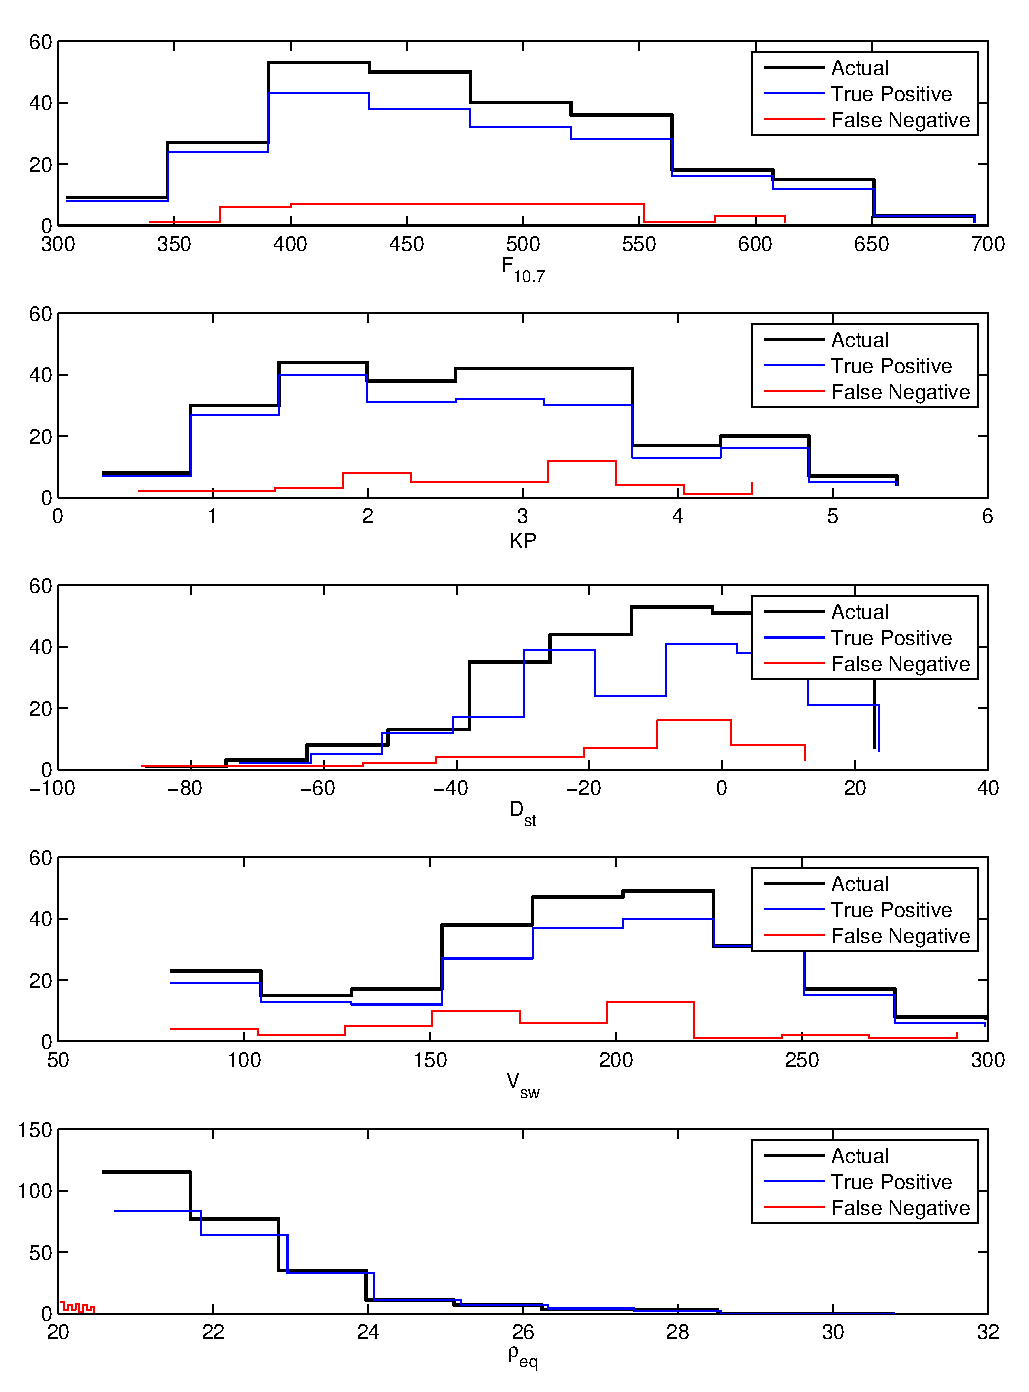
\includegraphics[width=1\linewidth]{Figures/CH5/NNBinaryOnset-hourly-withreq-hist.eps}
	\caption{Histogram of onset conditions for hourly \req\ events including \req\ as an input, binned by correctness of prediction.}
	\label{fig:OnsetWithreq-hist}
\end{figure}


\clearpage

\subsection{Forecasting} \label{sec:ForecastResults}

Using the full data set where each prediction was based on the previous four timesteps of inputs (\f, $K_p$, \dst, and $V_{SW}$) returned two models (daily and hourly). Both were tested with and without \req\ included as an input variable due to its more limited availability. All four confusion matrices are shown in Figure \ref{fig:OnsetFullWithreq}.

\begin{figure}[htp!]
	\centering
	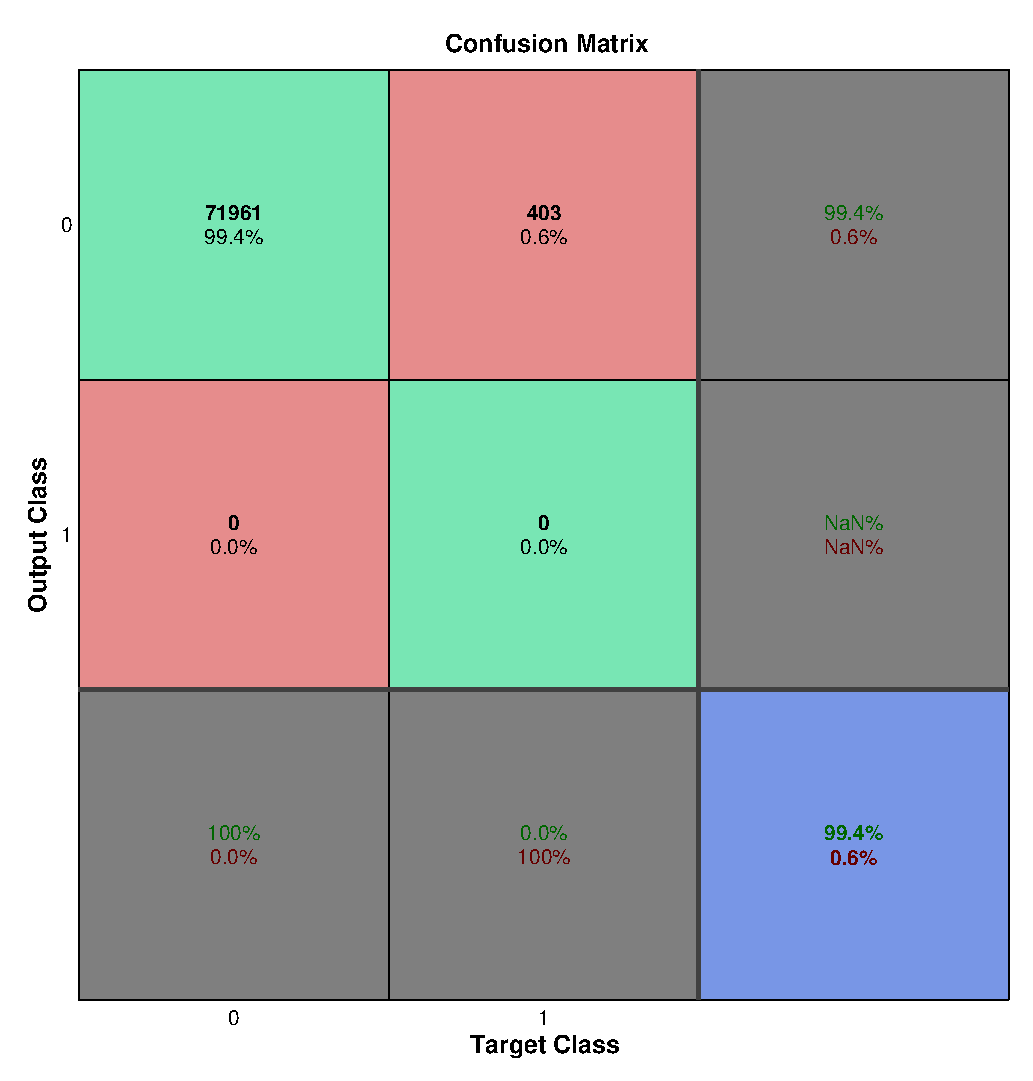
\includegraphics[width=0.45\linewidth]{Figures/CH5/NNBinaryOnset-full-hourly.eps}
	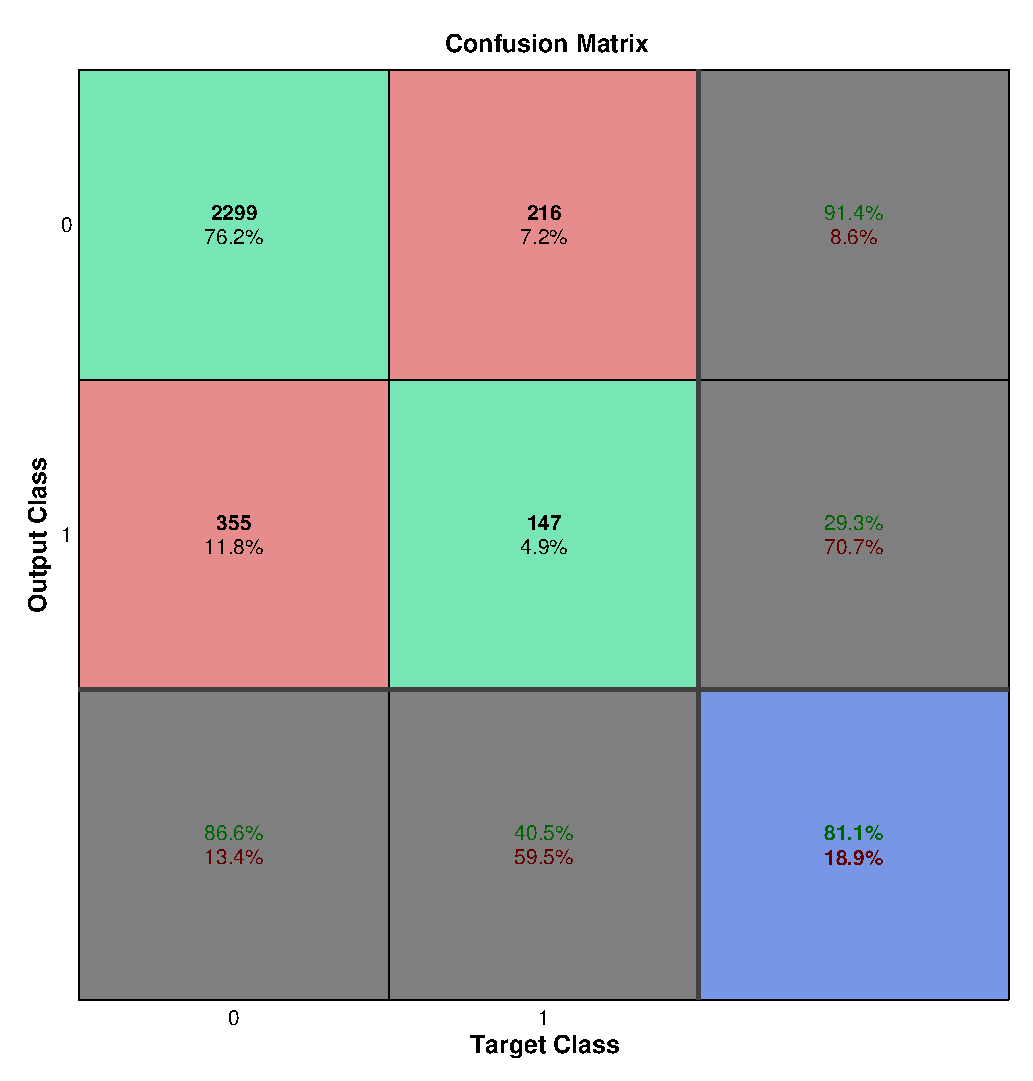
\includegraphics[width=0.45\linewidth]{Figures/CH5/NNBinaryOnset-full-daily.eps}
	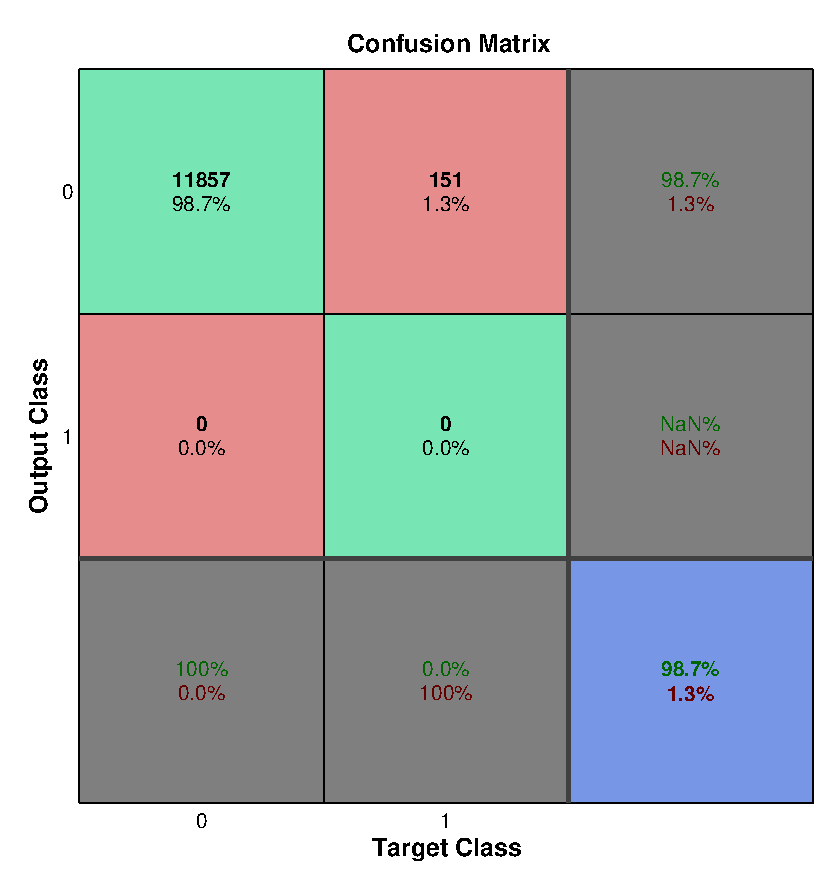
\includegraphics[width=0.45\linewidth]{Figures/CH5/NNBinaryOnset-full-hourly-withreq.eps}
	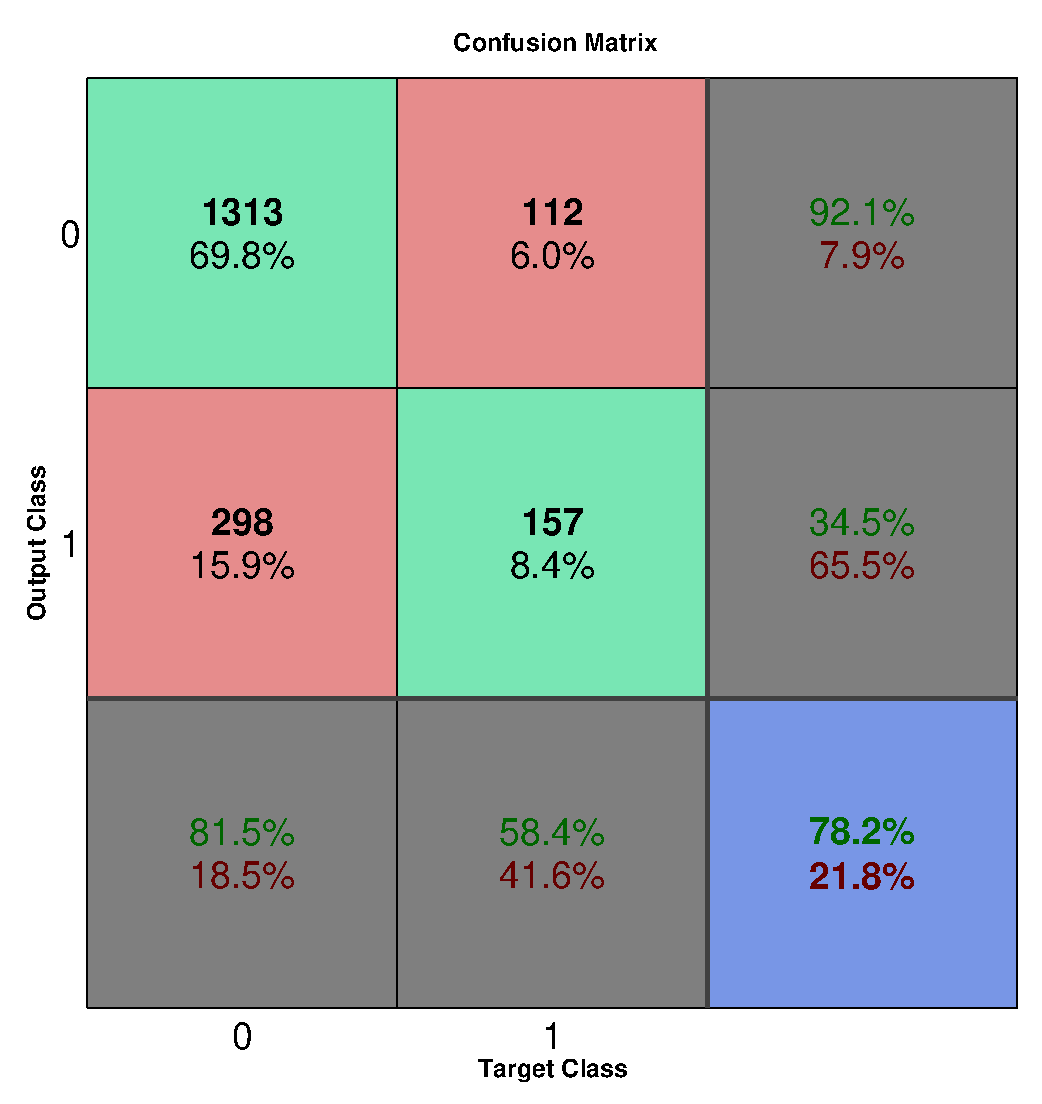
\includegraphics[width=0.45\linewidth]{Figures/CH5/NNBinaryOnset-full-daily-withreq.eps}
	\caption{Prediction confusion matrix for hourly (left column) and daily (right column) \req\ onset events, including \req\ as an input in the bottom row, and using entire timeseries with a four hour sliding window.}
	\label{fig:OnsetFullWithreq}
\end{figure}

It is seen that the selected weighting scheme is not sufficient to pick up hourly events without further tuning, but is overly aggressive with the daily values and ends up creating more false positives than truly correct predictions. That said, being able to predict 66\% of events a day in advance, at the cost of only half of the predicted onsets being accurate, is not completely useless. Again, the variables were broken down by value and correctness of prediction, this time taking the median value of each variable across the four-timestep bin. The resulting histograms are shown in Figure \ref{fig:OnsetWithreq-hist-full}.

\begin{figure}[htp!]
	\centering
	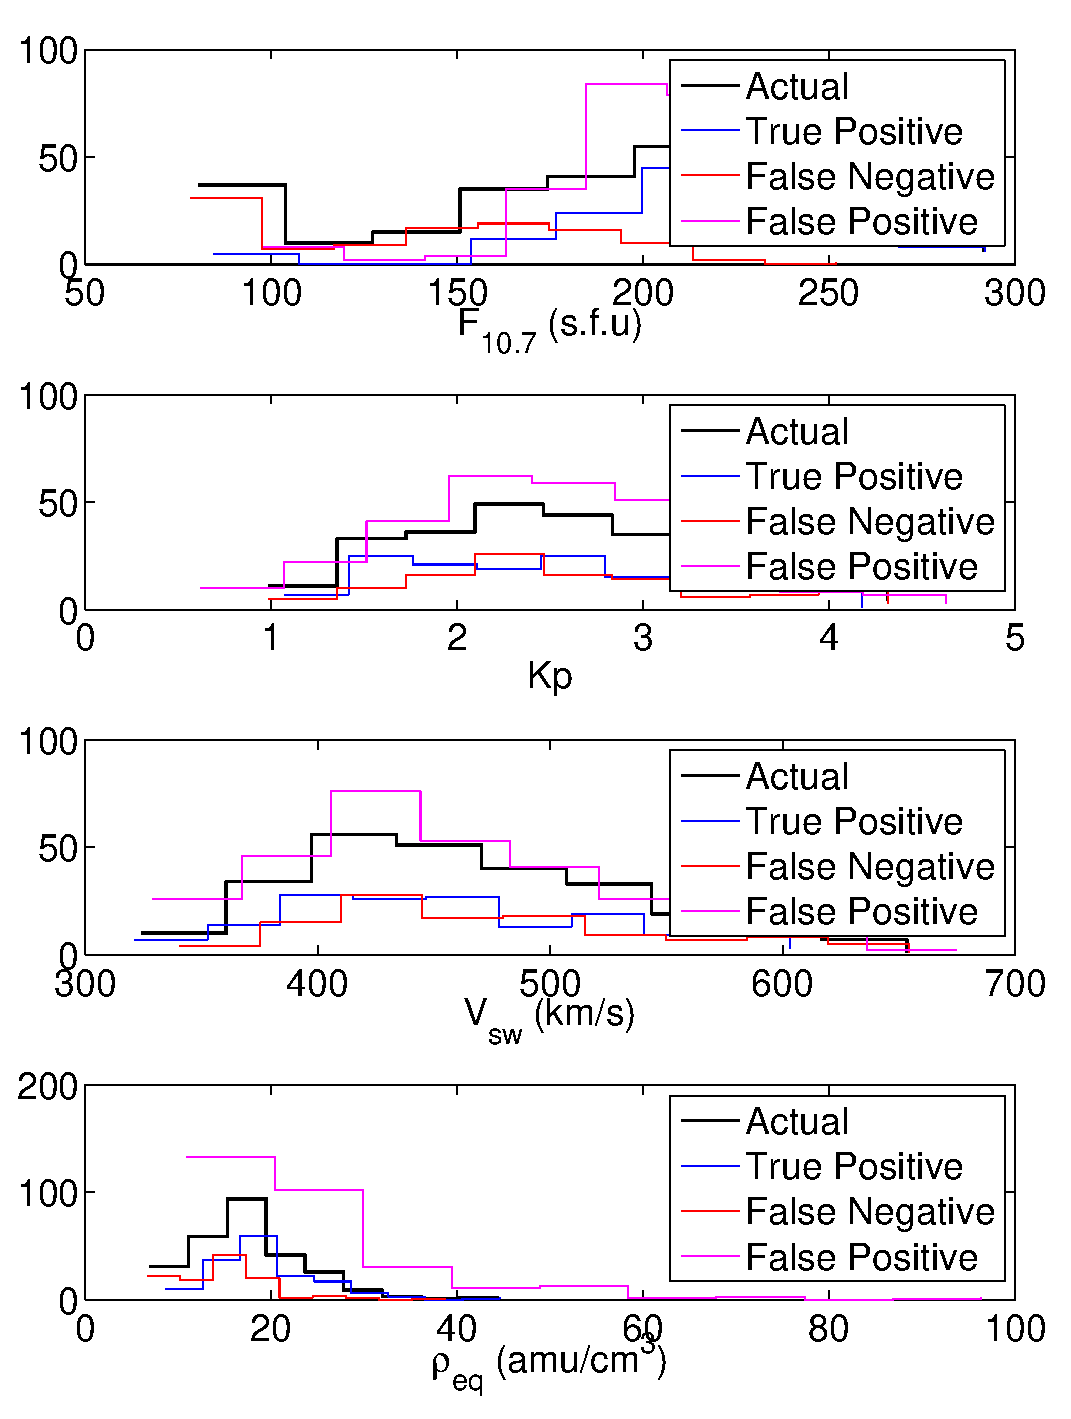
\includegraphics[width=1\linewidth]{Figures/CH5/NNBinaryOnset-full-daily-withreq-hist.eps}
	\caption{Histogram of onset conditions for daily \req\ events including \req\ as an input, binned by correctness of prediction.}
	\label{fig:OnsetWithreq-hist-full}
\end{figure}

This model seems to also miss predictions during periods of low solar activity and low density. Considering at least one value had to be less than 20, and one greater than 20, this might indicate that certain events are starting lower in value and barely crossing the threshold, and end up with poor predictions for it.  The model also shows that the false positives tend to follow the same distribution as the true onset values, suggesting that the model is picking up the structure but missing some other information that would determine whether \req\ actually sees a measured increase in value. As this is a first attempt at this sort of model, there is much room for refinement and improvement.


%\def\arraystretch{1.5}
% \begin{table}[h]
%	\begin{tabular}{CCCCCCCC}
% 		0 & 0 & 0 & 0 & 0 & 0 & 0 & 1 \\
% 		\hline
% 		B_{z_{\tau-7}} & B_{z_{\tau-6}} & B_{z_{\tau-5}} & B_{z_{\tau-4}} & B_{z_{\tau-3}} & B_{z_{\tau-2}} & B_{z_{\tau-1}} & B_{z_{\tau}}  \\
%		F_{10.7_{\tau-7}} & F_{10.7_{\tau-6}} & F_{10.7_{\tau-5}} & F_{10.7_{\tau-4}} & F_{10.7_{\tau-3}} & F_{10.7_{\tau-2}} & F_{10.7_{\tau-1}} & F_{10.7_{\tau}}  \\ 
%		K_{p_{\tau-7}} & K_{p_{\tau-6}} & K_{p_{\tau-5}} & K_{p_{\tau-4}} & K_{p_{\tau-3}} & K_{p_{\tau-2}} & K_{p_{\tau-1}} & K_{p_{\tau}}  \\
%		\rho_{eq_{\tau-7}} & \rho_{eq_{\tau-6}} & \rho_{eq_{\tau-5}} & \rho_{eq_{\tau-4}} & \rho_{eq_{\tau-3}} & \rho_{eq_{\tau-2}} & \rho_{eq_{\tau-1}} & \rho_{eq_{\tau}}  \\ 
% 		\hline
% 	\end{tabular}
% \end{table}